\documentclass[preview]{standalone}
\usepackage{amsmath}
\usepackage{tikz}
\usepackage{mathdots}
\usepackage{yhmath}
\usepackage{cancel}
\usepackage{color}
\usepackage{xcolor}
\usepackage{siunitx}
\usepackage{array}
\usepackage{multirow}
\usepackage{amssymb}
\usepackage{gensymb}
\usepackage{tabularx}
\usepackage{extarrows}
\usepackage{booktabs}
\usetikzlibrary{fadings}
\usetikzlibrary{patterns}
\usetikzlibrary{shadows.blur}
\usetikzlibrary{shapes}
\begin{document}
\begin{center}



\tikzset{every picture/.style={line width=0.75pt}} %set default line width to 0.75pt        

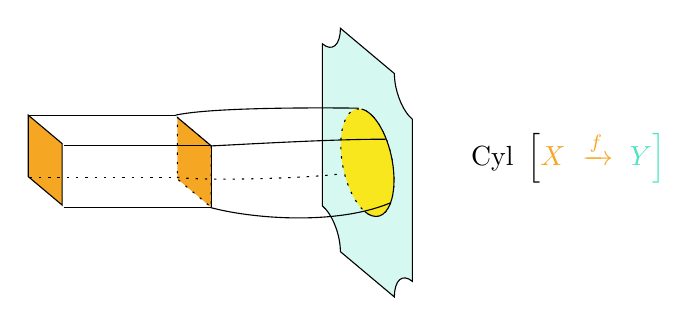
\begin{tikzpicture}[x=0.75pt,y=0.75pt,yscale=-1,xscale=1]
%uncomment if require: \path (0,158); %set diagram left start at 0, and has height of 158

%Shape: Plaque [id:dp8357345624430728] 
\draw  [fill={rgb, 255:red, 80; green, 227; blue, 194 }  ,fill opacity=0.24 ] (311.55,23) .. controls (316.35,27.02) and (320.23,23.66) .. (320.23,15.49) -- (346.25,37.33) .. controls (346.25,45.5) and (350.14,55.37) .. (354.93,59.39) -- (354.93,137.46) .. controls (350.14,133.44) and (346.25,136.8) .. (346.25,144.96) -- (320.23,123.13) .. controls (320.23,114.96) and (316.35,105.09) .. (311.55,101.07) -- cycle ;
%Shape: Arc [id:dp4295145729878398] 
\draw  [draw opacity=0][fill={rgb, 255:red, 248; green, 231; blue, 28 }  ,fill opacity=1 ][dash pattern={on 0.84pt off 2.51pt}] (344.42,99.6) .. controls (344.42,99.6) and (344.42,99.6) .. (344.42,99.6) .. controls (340.95,109.13) and (333.14,108.19) .. (326.96,97.49) .. controls (320.78,86.79) and (318.59,70.39) .. (322.06,60.86) .. controls (325.53,51.33) and (333.35,52.27) .. (339.52,62.97) .. controls (345.6,73.49) and (347.82,89.52) .. (344.59,99.11) -- (333.24,80.23) -- cycle ; \draw  [dash pattern={on 0.84pt off 2.51pt}] (344.42,99.6) .. controls (344.42,99.6) and (344.42,99.6) .. (344.42,99.6) .. controls (340.95,109.13) and (333.14,108.19) .. (326.96,97.49) .. controls (320.78,86.79) and (318.59,70.39) .. (322.06,60.86) .. controls (325.53,51.33) and (333.35,52.27) .. (339.52,62.97) .. controls (345.6,73.49) and (347.82,89.52) .. (344.59,99.11) ;  
%Shape: Rectangle [id:dp5307407676462352] 
\draw  [color={rgb, 255:red, 0; green, 0; blue, 0 }  ,draw opacity=1 ][fill={rgb, 255:red, 245; green, 166; blue, 35 }  ,fill opacity=1 ][dash pattern={on 0.84pt off 2.51pt}] (258,72.16) -- (258,101.78) -- (241.67,88.08) -- (241.67,58.46) -- cycle ;
%Curve Lines [id:da8431359818164164] 
\draw    (240.84,57.36) .. controls (256.65,53.92) and (300.9,53.65) .. (329,54) ;
%Curve Lines [id:da7780289161704352] 
\draw  [dash pattern={on 0.84pt off 2.51pt}]  (241.53,87.29) .. controls (254.82,89.23) and (307.19,87.74) .. (321.67,85.46) ;
%Shape: Arc [id:dp6431221609683067] 
\draw  [draw opacity=0][fill={rgb, 255:red, 248; green, 231; blue, 28 }  ,fill opacity=1 ] (330.44,54.44) .. controls (333.42,55.13) and (336.65,57.99) .. (339.52,62.97) .. controls (345.7,73.67) and (347.89,90.07) .. (344.42,99.6) .. controls (341.86,106.65) and (336.9,107.97) .. (332,103.84) -- (333.24,80.23) -- cycle ; \draw   (330.44,54.44) .. controls (333.42,55.13) and (336.65,57.99) .. (339.52,62.97) .. controls (345.7,73.67) and (347.89,90.07) .. (344.42,99.6) .. controls (341.86,106.65) and (336.9,107.97) .. (332,103.84) ;  
%Curve Lines [id:da47451449696150116] 
\draw    (258,72.16) .. controls (257.67,72.36) and (317.25,68.69) .. (342,69) ;
%Straight Lines [id:da7487812500514892] 
\draw    (241.67,58.46) -- (258,72.16) ;
%Straight Lines [id:da1805568826120123] 
\draw    (258,72.16) -- (258,101.78) ;
%Curve Lines [id:da24783965152706244] 
\draw    (257.42,101.81) .. controls (276.44,107.05) and (317.59,110.81) .. (344.42,99.6) ;
%Shape: Rectangle [id:dp394195741473198] 
\draw  [color={rgb, 255:red, 0; green, 0; blue, 0 }  ,draw opacity=1 ][fill={rgb, 255:red, 245; green, 166; blue, 35 }  ,fill opacity=1 ] (186.17,71.07) -- (186.17,100.69) -- (169.84,86.98) -- (169.84,57.36) -- cycle ;
%Straight Lines [id:da4183715374083836] 
\draw    (169.84,57.36) -- (240.84,57.36) ;
%Straight Lines [id:da6995682946561381] 
\draw    (187,72.16) -- (258,72.16) ;
%Straight Lines [id:da17317067644135342] 
\draw    (187,101.78) -- (258,101.78) ;
%Straight Lines [id:da749473570975463] 
\draw  [dash pattern={on 0.84pt off 2.51pt}]  (170.53,87.29) -- (241.53,87.29) ;

% Text Node
\draw (382,64.4) node [anchor=north west][inner sep=0.75pt]    {$\mathrm{Cyl} \ \left[\color[rgb]{0.96,0.65,0.14}{X} \ \xrightarrow{f} \ \color[rgb]{0.31,0.89,0.76}{Y}\right]$};


\end{tikzpicture}

\end{center}
\end{document}
